% state/pose3_and_cant.tex

\chapter{Pose3, Cant, and Spatial Railway State}

% ============================================================
\section{Motivation}
% ============================================================

\begin{remark}
Classical railway alignment models are based on planar geometry.
They describe the track centerline as a curve
\[
\gamma : s \mapsto (x(s),y(s)).
\]
\end{remark}

\begin{remark}
However, real railway systems are inherently three-dimensional.
In particular, the rotation of the track cross-section, commonly
described through cant, plays a fundamental role for vehicle dynamics
and operational behaviour
\cite{Klein1998Trassierung,EN13803_2017}.
\end{remark}

\begin{remark}
The pose3 formulation also opens the possibility of describing the
motion of physically relevant vehicle reference points, such as the
vehicle centre of gravity, instead of modelling only the track
centerline.

Such ideas have occasionally appeared in advanced railway engineering
concepts and patent literature
\cite{Hasslinger2002Schwerpunkt}.
\end{remark}

\begin{remark}
This motivates the introduction of an extended runtime state description,
referred to as \emph{pose3}, which augments planar alignment geometry by
vertical and rotational information.
\end{remark}

\begin{figure}[h]
\centering
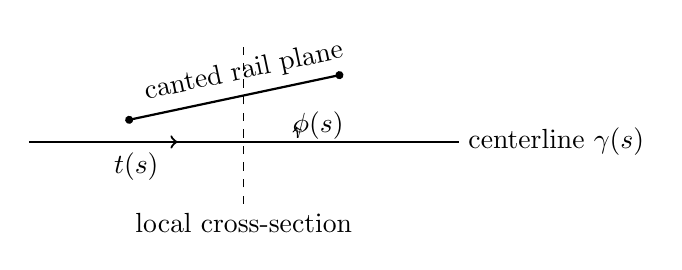
\begin{tikzpicture}[scale=1.05]

% track centerline
\draw[thick] (-2.6,0) -- (2.6,0);
\node[right] at (2.6,0) {centerline $\gamma(s)$};

% tangent arrow
\draw[->, thick] (-1.8,0) -- (-0.8,0) node[midway, below] {$t(s)$};

% cross section, canted
\draw[thick, rotate around={12:(0,0)}] (-1.3,0.55) -- (1.3,0.55);
\fill[rotate around={12:(0,0)}] (-1.3,0.55) circle (1.4pt);
\fill[rotate around={12:(0,0)}] (1.3,0.55) circle (1.4pt);
\node[rotate=12] at (0,0.85) {canted rail plane};

% rotation arc
\draw[->] (0.65,0.05) arc[start angle=0,end angle=12,radius=0.65];
\node at (0.9,0.2) {$\phi(s)$};

% vertical hint
\draw[dashed] (0,-0.75) -- (0,1.15);
\node[below] at (0,-0.75) {local cross-section};

\end{tikzpicture}

\caption{Pose3 extends the planar centerline state by vertical and
rotational information. In AIM, the roll angle $\phi(s)$ is derived from
cant and gauge rather than stored as persistent truth.}
\end{figure}

% ============================================================
\section{Pose2 Revisited}
% ============================================================

\begin{definition}[Pose2]
The planar pose of a curve is defined as
\[
\mathrm{pose2}(s)
=
\bigl(
\gamma(s), \theta(s)
\bigr),
\]
where
\[
\gamma(s)\in\R^2, \qquad \theta(s)\in\R.
\]
\end{definition}

\begin{remark}
The evolution of pose2 is governed by
\[
\theta'(s)=\kappa(s),
\qquad
\gamma'(s)=(\cos\theta(s),\sin\theta(s)).
\]
\end{remark}

\begin{remark}
This is the planar reconstruction principle underlying the cGeom band
of the sparse alignment model.
\end{remark}

% ============================================================
\section{Cant as Superelevation Band}
% ============================================================

\begin{definition}[Cant]
Within AIM, cant is represented as a rail height difference
\[
u(s),
\]
not as a stored roll angle.
\end{definition}

\begin{remark}
This follows railway engineering practice, where cant is commonly given
as height difference between rails.
\end{remark}

\begin{definition}[Derived roll angle]
Given a gauge value \(g_{\mathrm{auge}}\), the corresponding roll angle is
derived by
\[
\phi(s)
=
\arctan\!\left(
\frac{u(s)}{g_{\mathrm{auge}}}
\right).
\]
\end{definition}

\begin{remark}
Thus, the roll angle depends on both cant and gauge. It is therefore a
derived state quantity rather than persistent cant data.
\end{remark}

\begin{remark}
The cant angle influences lateral acceleration, cant deficiency, and
load distribution
\cite{Klein1998Trassierung,EN13803_2017}.
\end{remark}

% ============================================================
\subsection{Cant Reference Axis and Centerline Convention}
% ============================================================

\begin{remark}
In standard railway handling, cant is often specified by rotating the
track plane around a relevant rail or by defining a height difference
between rails.
\end{remark}

\begin{remark}
The AIM state model uses the centerline point as the primary reference
point of the alignment.
Thus, cant must be translated into a centerline-based representation
before it is coupled to profile, pose3, and optimization.
\end{remark}

\begin{definition}[Cant reference convention]
A cant convention specifies:
\begin{itemize}
\item the reference axis of rotation,
\item the sign convention of cant,
\item the relation between rail height difference and roll angle,
\item and the induced vertical offset of the centerline.
\end{itemize}
\end{definition}

\begin{remark}
This distinction is relevant in special cases such as track scissors,
cant ramps, and overlapping transition zones, where the cant definition
may influence the effective profile or gradient assigned to the
centerline.
\end{remark}

\begin{remark}
For implementation, AIM treats cant not merely as an isolated value, but
as a band whose reference convention must be known when transforming
between rail-based construction data and centerline-based modelling.
\end{remark}

\begin{definition}[Cant rate]
The derivative
\[
\phi'(s)
\]
describes the rate of change of the derived roll angle along the track.
\end{definition}

\begin{remark}
Cant rate is not merely a geometric quantity, but an engineering
quantity constrained by operational and comfort-related requirements
\cite{EN13803_2017}.
\end{remark}

% ============================================================
\section{Persistent Model versus Runtime State}
% ============================================================

\begin{principle}[Runtime pose3 principle]
Pose3 is not persistent truth within AIM.
It is a runtime-derived spatial state.
\end{principle}

\begin{remark}
The persistent sparse model stores:
\begin{itemize}
\item cGeom as pose2-driven curvature geometry,
\item cant as a longitudinal superelevation band,
\item profile as a separate height band.
\end{itemize}
\end{remark}

\begin{remark}
Pose3 is derived dynamically from these bands by runtime evaluation
services.
\end{remark}

\begin{remark}
This avoids redundant storage of three-dimensional points, roll angles,
and derived spatial frames.
It also avoids synchronization instability between geometry, cant, and
profile.
\end{remark}

\begin{summary}
The intelligence of the AIM state model does not reside in a stored
pose3 object, but in the mathematical services that evaluate pose3 from
sparse longitudinal bands.
\end{summary}

% ============================================================
\section{Pose3 Definition}
% ============================================================

\begin{definition}[Runtime Pose3]
The spatial railway state is defined as
\[
\mathrm{pose3}(s)
=
\bigl(
\Gamma(s),
\mathbf{t}(s),
\phi(s)
\bigr),
\]
where:
\begin{itemize}
\item \(\Gamma(s)\) is the reconstructed three-dimensional centerline
point,
\item \(\mathbf{t}(s)\) is the spatial tangent direction,
\item \(\phi(s)\) is the derived roll angle.
\end{itemize}
\end{definition}

\begin{remark}
In the projected engineering setting, \(\Gamma(s)\) is obtained from
planar pose2 and profile evaluation.
\end{remark}

\begin{remark}
Pose3 captures both geometric and dynamically relevant aspects of the
track, but remains a derived runtime state.
\end{remark}

\begin{remark}
When a rail-based cant convention is used in source data, the
centerline-consistent state must be resolved during import,
normalization, or model construction.
\end{remark}

% ============================================================
\section{State Evolution}
% ============================================================

\begin{proposition}[Projected pose3 evolution]
In a projected engineering coordinate system, the runtime pose3 state is
derived from:
\[
\begin{aligned}
\gamma'(s) &= (\cos\theta(s),\sin\theta(s)), \\
\theta'(s) &= \kappa(s), \\
z(s)       &= p(s), \\
\phi(s)    &= \arctan\!\left(\frac{u(s)}{g_{\mathrm{auge}}}\right),
\end{aligned}
\]
where \(p(s)\) denotes profile height and \(u(s)\) denotes cant as rail
height difference.
\end{proposition}

\begin{remark}
Thus, pose3 is not governed by one monolithic state equation.
It is assembled from synchronized evaluations of cGeom, profile, and
cant.
\end{remark}

% ============================================================
\section{Reconstruction Principle}
% ============================================================

\begin{proposition}
Given:
\[
\kappa(s), \quad p(s), \quad u(s),
\]
together with initial pose2 data and gauge information, the runtime
pose3 state is determined by evaluation.
\end{proposition}

\begin{remark}
This differs from storing pose3 directly.
The sparse model stores the ingredients; pose3 is reconstructed when
needed.
\end{remark}

% ============================================================
\section{Relation to Physical Quantities}
% ============================================================

\subsection{Effective Lateral Acceleration}

\begin{definition}
In the planar engineering approximation, effective lateral acceleration
is given by
\[
a_{\mathrm{eff}}(s)
=
v^2 \kappa(s) - g \sin\phi(s).
\]
\end{definition}

\begin{remark}
This quantity determines passenger comfort and safety and expresses the
basic coupling between curvature and cant in operational railway design
\cite{Klein1998Trassierung,EN13803_2017}.
\end{remark}

\subsection{Jerk}

\begin{definition}
The jerk is given by
\[
j(s)
=
v^3 \kappa'(s) - g v \cos\phi(s)\,\phi'(s).
\]
\end{definition}

\begin{remark}
The jerk measures the rate of change of acceleration and is a key
criterion for comfort. This is one of the main reasons why curvature and
cant development cannot be specified independently in high-quality
alignment design
\cite{Mieloszyk2012Transition,Koc2017SmoothedEnds,Koc2019Operational}.
\end{remark}

% ============================================================
\section{Interpretation as Evaluation System}
% ============================================================

\begin{remark}
The pose3 model can be interpreted as an evaluation system:
\[
\begin{aligned}
\text{persistent bands:} &\quad \mathrm{cGeom},\ u,\ p, \\
\text{runtime state:}   &\quad \mathrm{pose3}.
\end{aligned}
\]
\end{remark}

\begin{remark}
This formulation provides a natural bridge to simulation, visualization,
validation, and optimization methods.
\end{remark}

\begin{remark}
It is also consistent with the broader optimization-oriented view of
alignment modelling proposed in railway alignment research
\cite{Kufver1997MathematicalDescription,Kufver2000RailwayAlignment}.
\end{remark}

% ============================================================
\section{Cant and Curvature Coupling}
% ============================================================

\begin{remark}
Curvature and cant are not independent in engineering interpretation.
They jointly determine dynamic behaviour.
\end{remark}

\begin{definition}[Equilibrium condition]
A perfectly balanced design satisfies
\[
v^2 \kappa(s) = g \sin\phi(s).
\]
\end{definition}

\begin{remark}
In practice, deviations from this condition are allowed but must remain
within regulatory limits. This is the mathematical expression of the
cant-balance logic used in railway design standards
\cite{EN13803_2017,Klein1998Trassierung}.
\end{remark}

\begin{remark}
The persistent model keeps cGeom and cant as separate synchronized
bands. Their coupling is evaluated dynamically rather than stored
redundantly.
\end{remark}

% ============================================================
\section{Towards Schwerpunkt-Trassierung}
% ============================================================

\begin{remark}
The pose3 formulation enables a reinterpretation of alignment design.
Instead of designing geometry alone, one designs a spatial state
trajectory.
\end{remark}

\begin{remark}
In particular, the concept of \emph{Schwerpunkt-Trassierung} can be
understood as the design of a trajectory that optimally balances
curvature, cant, and dynamic response.
\end{remark}

\begin{remark}
In the sparse AIM model, cant may remain coupled to the normalized
curvature family, while curvature itself may receive additional
correction terms for advanced modelling concepts.
\end{remark}

\RESEARCH{Formal definition of Schwerpunkt-based alignment design.}

\OPEN{Integration of vehicle dynamics into the pose3 framework.}

% ============================================================
\section{Relation to Existing Standards}
% ============================================================

\begin{remark}
Existing railway design standards typically prescribe:
\begin{itemize}
\item limits on curvature,
\item limits on cant,
\item limits on cant gradient.
\end{itemize}
\end{remark}

\begin{remark}
These rules can be interpreted as constraints on the runtime pose3 state
and its derivatives \cite{EN13803_2017}.
\end{remark}

\begin{remark}
From this perspective, pose3 does not contradict existing railway
standards, but provides a mathematical structure in which such rules can
be represented coherently.
\end{remark}

\begin{remark}
The purpose of the pose3 formulation is not to replace such standards,
but to make their geometric consequences explicit. In particular,
rail-based cant rules must be converted consistently when the internal
model uses the centerline as its reference geometry.
\end{remark}

% ============================================================
\section{Connection to the AIM Framework}
% ============================================================

\begin{summary}
Pose3 extends planar alignment modelling to spatial railway state
evaluation.

Within AIM, pose3 is not persistent truth. It is derived at runtime from
cGeom, cant, profile, and coordinate services.

This provides:
\begin{itemize}
\item a unified runtime interpretation of geometry and dynamics,
\item a natural interface to validation and optimization methods,
\item a foundation for advanced concepts such as
Schwerpunkt-Trassierung.
\end{itemize}
\end{summary}
